\documentclass[UTF8,letterpaper,twocolumn,11pt,fontset=fandol]{ctexart}
\usepackage[margin=0.73in,columnsep=0.27in]{geometry}
\usepackage[hyphens]{url}
\usepackage{graphicx}
\urlstyle{rm}
\def\UrlFont{\rm}
\usepackage{natbib}
\usepackage{caption}
\usepackage{booktabs}
\frenchspacing
\bibliographystyle{aaai2027}\setlength{\tabcolsep}{3pt}
\setcounter{secnumdepth}{0}
\title{哪种剂量预测器适合当前队列？\\面向放疗模型选择的可审计智能体设计}
\author{匿名稿}
\date{}
\begin{document}
\maketitle

\begin{abstract}
放疗剂量预测需要同时准确估计靶区覆盖和邻近器官的受照剂量。即便治疗部位相同，不同患者可用于训练和评价的解剖结构也有差异。我们提出一种调用工具的智能体，用于为给定队列选择预测模型。智能体拟根据靶区几何、轮廓勾画情况和剂量梯度提出 SearchedNet 架构及训练超参数的调整方案，再通过独立的匹配对照检验排除存在质量疑点的记录能否改善预测。为评估选择该搜索空间的依据，我们在 OpenKBP 留出的 100 名头颈部测试患者上比较了固定三维 U-Net 与已有搜索配置 NAS-29。NAS-29 将平均剂量误差从 2.654 Gy 降至 2.555 Gy，将汇总剂量体积直方图（DVH）误差从 1.809 Gy 降至 1.663 Gy。靶区覆盖估计有所改善，脊髓近最大剂量误差却有所增加。这些结果支持在评价 SearchedNet 配置时同时考察体素剂量和分结构终点。选型智能体的实现与评估属于后续工作。
\end{abstract}

\section{引言}
在头颈部放疗中，为保护脊髓，剂量有时需要在离开靶区后很短的距离内从处方水平迅速下降。模型可能准确还原大部分剂量场，却在最靠近靶区的一小段脊髓上产生较大偏差。OpenKBP 通过两项互补指标评价预测：基于体素的剂量分数，以及根据靶区和器官终点计算的剂量体积直方图（DVH）分数\citep{openkbp}。用于模型选择时，即使平均体素误差下降，也需要进一步检查改善来自哪些结构，以及哪些结构的预测仍有偏差。

给定计划 CT、计划靶区（PTV）及危及器官（OAR）轮廓，我们的目标是预测以戈瑞（Gy）为单位的三维参考剂量。将预测结果转化为可实际投照的计划，还需在设备约束和计划目标下求解优化问题\citep{planning}。拟议的智能体参与模型开发；推理时，选定网络接收带轮廓的 CT，输出剂量场。

U-Net 是生物医学影像中常用的编码器–解码器架构\citep{unet}。在头颈部剂量预测中，已有研究将密集连接与空洞卷积引入三维 U-Net\citep{gronberg}。训练会调整网络权重，而感受野设计、分辨率变化方式和解码算子均已预先确定。这些选择是否合适，可能与靶区大小、靶区至器官的距离及器官勾画率有关。我们建议将这些关系转化为可检验的假设，在训练前明确拟替换的算子及相应的评价终点。

我们将 SearchedNet 作为初始候选模型族，因为其编解码算子可在共同的拓扑结构中替换。为评估这一选择，我们在相同训练方案下比较 LENAS 搜索空间中的配置 NAS-29\citep{lenas} 与固定三维 U-Net。除报告队列级剂量分数和 DVH 分数外，我们还通过累积 DVH 曲线比较两种模型在靶区覆盖和器官受照剂量上的预测差异。NAS-29 在该队列上的两项汇总误差均较低，由此引出下一步问题：在相同的搜索预算下，以训练队列测量为依据提出候选，能否比在同一空间内直接采样找到更好的预测器？

\section{问题定义与相关研究}
对患者 $i$，令 $X_i$ 表示对齐到同一网格的 CT、靶区和器官掩膜，$D_i$ 为参考剂量（Gy），$M_i$ 为可能接受剂量的体素集合。预测器 $f_\theta(X_i)$ 对每个体素输出一个剂量值。该患者的空间剂量误差为
\begin{equation}
 e_i=\frac{1}{|M_i|}\sum_{v\in M_i}
 \left|f_\theta(X_i)_v-D_{iv}\right|.
\end{equation}
即使器官位于剂量快速变化的区域，其掩膜仍可确定解剖范围。累积 DVH 表示某结构中接受至少给定剂量的体积分数。两个剂量场可以具有相似的 DVH，却把剂量分配到不同的体素；小器官的高剂量端也可能有较大偏差，却对 $e_i$ 影响很小。因此，选型记录同时保留空间误差和 DVH 误差。

已有工作从不同环节使医学影像模型适应数据。在分割任务中，nnU-Net 根据数据集特性配置预处理、网络和训练流程\citep{nnunet}。在剂量预测中，nnDoseNet 将这一思路用于连续剂量回归，并比较不同训练配置\citep{nndose}。DoseDiff 以距离图将解剖几何信息直接引入预测器\citep{dosediff}。LENAS 搜索网络模块，利用集成和知识蒸馏发挥不同预测器的互补作用\citep{lenas}。本文关注选型过程：将实际测得的队列特征与病例纳入、架构或训练参数的一项具体改动关联起来，并记录支持或质疑该选择的试验。

\subsection{训练队列中的轮廓差异}
OpenKBP 为头颈部病例提供合成参考计划，因此预测误差衡量的是与该基准计划方案的一致程度。数据划分为训练 200 例、验证 40 例、测试 100 例\citep{openkbp}。表~\ref{tab:cohort} 汇总了训练轮廓。体积由勾画体素数乘以该患者的单体素体积，再换算为毫升。全部 200 例均有 70 Gy 靶区，最大靶区体积超过最小值的百倍。仅 81 例有食管轮廓。缺少轮廓既影响模型输入，也减少能够评价食管剂量的病例数；对未勾画食管的患者，不能据此推断其预测误差。

\begin{table}[t]
\centering\small
\begin{tabular}{lrrr}
\toprule
结构 & 例数 & 中位数（mL） & 范围（mL）\\
\midrule
PTV70 & 200 & 291.15 & 9.02--1245.13\\
脑干 & 182 & 25.42 & 4.87--47.54\\
脊髓 & 188 & 25.58 & 5.34--57.04\\
食管 & 81 & 11.68 & 2.20--40.87\\
喉 & 100 & 24.08 & 0.53--85.84\\
\bottomrule
\end{tabular}
\caption{部分训练结构的轮廓统计。每行仅纳入勾画该结构的患者，每例贡献一个体积观测。}
\label{tab:cohort}
\end{table}

拟议工具还将测量两类特征。其一是每个已勾画 OAR 至所有 PTV 并集的最短距离（mm），以及交叠体积占该器官体积的比例。其二是按各轴实际体素间距，估计器官边界内侧 3 mm 带状区域的参考剂量梯度（Gy/mm）。工具应同时报告有效病例数和体素数，因为薄边界带的高分位数可能只取决于少数观测。上述量将作为搜索依据；仅凭已测得的轮廓体积，还不能判断哪种算子更适合小靶区。

\section{面向模型开发的智能体设计}
拟议控制器接收患者清单、输出目录和计算预算。本地工具负责处理影像、测量队列特征和执行训练，并返回统计量、实际生效的配置、作业编号和产物位置。这些记录支持三项决策：哪些病例可用于训练，哪些架构与超参数组合值得晋级，以及更严格的病例纳入清单能否使选定模型获益。已完成的基线实验采用原始训练集和人工指定的配置。

\begin{table*}[t]
\centering\small
\begin{tabular}{lp{2.65in}ll}
\toprule
单元位置 & 可选算子 & NAS-29 编码器 & NAS-29 解码器\\
\midrule
主路第一项 & 恒等、标准卷积、深度可分离卷积、空洞卷积、SE 通道加权 & 恒等 & 深度可分离卷积\\
主路第二项 & 同上五项，可独立选择 & 空洞卷积 & 深度可分离卷积\\
局部旁路 & 恒等或置零 & 置零 & 置零\\
编码器出口 & 平均池化、最大池化，或步长为 2 的标准、深度可分离、空洞、SE 卷积 & 深度可分离卷积 & ---\\
解码器出口 & 标准、深度可分离、空洞、SE 转置卷积，或卷积后接三线性插值 & --- & 卷积后三线性插值\\
\bottomrule
\end{tabular}
\caption{SearchedNet 的完整算子选项。SE 指挤压与激励通道加权。算子名称对应激活和归一化封装内的权重运算。右两列给出已完成实验中 NAS-29 的八个选择。}
\label{tab:ops}
\end{table*}

\subsection{训练记录的筛选}
数据准备工具将检查参考剂量是否可读、数值是否有限，CT、剂量和掩膜是否共用坐标系，以及可给剂量掩膜是否非空。转换失败时，按已记录的程序从源文件重新转换。无法修复的记录连同源文件核查结果一并隔离；经确认的重复病例仅保留一份。由此得到的合格训练池 $B$ 可追溯至原始清单。

第二轮审查尚可使用、但可能干扰训练的记录。患者级特征包括靶区体积、勾画情况、体素间距、剂量分位数和边界梯度。仅在训练集上以中位数填补缺失值，保留缺失标志，按四分位距缩放后，对 $k=2,\ldots,5$ 拟合 $k$ 中心点聚类，以平均轮廓系数选择 $k$。若病例至中心点的距离超出簇内距离中位数三个中位绝对偏差，则提名复核。簇内少于五例、离散度为零或聚类缺乏支持时，标为证据不足。在五次固定种子的 80\% 子样本拟合中，至少四次一致提名，且另有独立核实的质量疑点（如源元数据与转换后剂量单位不符），才进入候选清单。

解剖罕见的患者可能远离任何聚类中心，恰恰也是模型需要学习的病例。工具须保护人数少的预设亚组及罕见勾画器官的最后样例，记录筛选前后的覆盖情况。暂拟排除的病例不超过 $B$ 的 5\%，也允许一个都不排除。在读取验证成绩前冻结唯一的候选集合 $E$。待完成模型选择后，再固定网络和训练参数，对照 $B$ 与筛选池 $F=B\setminus E$。

\subsection{各位置的算子选择}
SearchedNet 采用固定 U 形拓扑，编码器和解码器分别在四个分辨率上复用各自的单元结构，每层独立学习权重。单元先对输入做预处理，再将其送入两条路径：主路串联两个算子，局部旁路经过第三个算子。两路逐元素相加，再经第四个算子改变分辨率。局部旁路与编解码器之间固定的特征拼接各有其作用。两类单元一共需要指定八个位置（表~\ref{tab:ops}）。



控制器将以 NAS-29 为起点提出两个不同变体。每项提案都须指明待更改的位置、提案所依据的测量（含单位和分母）、备选算子，以及可用于检验假设的终点。例如，若小器官附近剂量梯度较陡，可尝试保留解码器局部旁路以保留边界信息，试验仅改变这一处。若总体剂量误差降低而小器官误差上升，则会削弱原先的解释。若靶区与器官的间距变化较大，则可优先试验将编码器首个算子更换为空洞卷积。队列测量决定哪些试验值得优先开展，验证结果决定哪些配置晋级。

\begin{table*}[t]
\centering\small
\begin{tabular}{p{1.02in}p{3.36in}p{2.06in}}
\toprule
阶段 & 提示词节选 & 返回或核验的证据\\
\midrule
分析队列 & 计算边界剂量梯度（Gy/mm），报告患者数、有效邻域体素数、离散程度及器官缺失处理规则。 & 训练清单版本、分结构统计、单位和分母。\\
复核病例 & 对稳定离群者重新读取源数据，记录独立质量疑点及应予保留的合理解释。 & 逐例处置、源文件核查、聚类稳定性及覆盖变化。\\
选择算子 & 填写全部八项配置。对每个改动位置，指出备选算子和可以推翻假设的验证结果。 & 有序结构配置、证据编号、对照架构及试验设计。\\
核验试验 & 核对实际算子，读回优化器中的学习率和权重衰减，测量训练一步后的显存峰值。 & 实际结构、优化器参数组、硬件测量及可行性。\\
选择训练数据 & 固定胜出组合及更新步数，对照两份冻结清单。报告各患者配对差值和保护亚组人数。 & 作业编号、检查点指纹、亚组结果和正式清单。\\
\bottomrule
\end{tabular}
\caption{智能体提示词节选。工具返回的记录可用于核对控制器对其决策的解释。已报告的基线实验未运行该控制器。}
\label{tab:prompts}
\end{table*}

\subsection{计算预算约束下的联合搜索}
调度前，硬件工具将报告可用设备、支持的计算后端和精度、内存、CPU 容量及存储空间。随后，每个候选模型均以完整分辨率的小批量数据执行前向计算、反向传播和一次优化更新，以确定各模型均可运行的全局批量大小，并核验实际优化参数。例如，现有 Adam 实现的一个分支会在内部指定权重衰减值，两次设置不同衰减值的请求可能得到相同的优化器。控制器可读取实际参数组、合并重复试验，并报告有效搜索范围。

默认比较三个结构、两个初始学习率（$10^{-4}$ 和 $3\times10^{-4}$）及两个权重衰减值（0 和 $3\times10^{-5}$），共十二种组合。按 PTV 体积四分位分层，从 $B$ 中固定抽取 48 名患者，每种组合训练 1,000 步。首轮试验前即确定患者清单及稀有器官覆盖率。各候选共用增强方式、初始化规则、样本抽取预算和 40 人验证清单。每 500 步验证一次，以最佳验证剂量分数排序，平局依次比较 DVH 误差、参数量和固定组合编号。

排名前两位的组合可能采用相同架构，分别在 $B$ 上从头训练 5,000 步，仅按该阶段验证结果决选。若 $E$ 非空且预算允许，再以相同种子、全局批量和调度规则在 $F$ 上训练胜出组合 5,000 步。只有同时满足下列条件才采用 $F$：按患者配对自助重抽样所得剂量误差差值（$F-B$）的 95\% 区间上界低于零；汇总 DVH 误差未升高；预定的小体积和高梯度亚组各至少有五名可评价患者，且组内平均剂量误差均未升高。否则保留 $B$。这种对照只能检验整项筛选策略，无法据此认定某个病例造成了性能变化。

最后，在选定清单上将胜出组合从头训练 80,000 步。搜索与正式训练共需 102,000 次优化更新，含可选筛选对照时为 107,000 次。数据分析、验证和重试还需额外时间。控制器先预留正式训练预算，再视资源缩减参数网格。失败和未完成的作业与成功记录一并保留，以便审查者知道显存是否限制了可选模型。

\subsection{提示词与决策溯源}
十三份提示词规定了从队列分析、病例复核到训练执行、检查点选择的决策和工具调用。表~\ref{tab:prompts} 列出代表性指令及其要求的证据。例如，推荐某个算子时，控制器须指出备选算子，并说明何种结果会削弱其推荐理由；训练工具随后须确认实际实例化的算子。审查者可据此核对提案与实际受评估的干预是否一致。



面向 Bridge 讨论，我们建议用小型溯源图表示实验轨迹。测量节点记录队列、统计量和单位；提案关联支持它的测量及拟改动的配置；训练事件将实际算子、优化器和清单绑定到检查点；评价事件再将检查点与指定患者集上的成绩关联起来。沿图回溯即可同时找到胜出的组合及被淘汰的对照。图可由实际工具事件构成，无须存放患者扫描或临床身份信息。

审查者可以通过两类查询使用该图。要解释解码器旁路的选择，控制器应检索提出该改动所依据的测量，以及只更改该位置的试验。要评价同一模型对脊髓受照剂量的估计，则应检索脊髓终点、对照模型和可评价患者数。若备选配置在评价前运行失败，溯源记录应定位到失败作业；有关该算子优势的解释仍属未经检验的假设。

\section{已完成的 OpenKBP 实验}
\begin{table*}[t]
\centering\small
\begin{tabular}{lrrrrrr}
\toprule
& \multicolumn{3}{c}{3D U-Net} & \multicolumn{3}{c}{NAS-29}\\
\cmidrule(lr){2-4}\cmidrule(lr){5-7}
指标与统计单位 & 均值 & 标准差 & 范围 & 均值 & 标准差 & 范围\\
\midrule
剂量误差，100 例 & 2.654 & 1.095 & 1.301--7.847 & 2.555 & 1.042 & 1.251--7.286\\
DVH 误差，1,783 项 & 1.809 & 2.066 & 0.001--26.396 & 1.663 & 1.991 & 0.001--25.216\\
患者级平均 DVH 误差，100 例 & 1.824 & 1.276 & 0.800--11.997 & 1.663 & 1.174 & 0.750--11.667\\
\bottomrule
\end{tabular}
\caption{OpenKBP 留出测试集结果。误差单位为 Gy，越低越好。前两行为基准指标，第三行赋予每位患者相同权重，用于解释病例分析。}
\label{tab:results}
\end{table*}

\subsection{输入与训练方案}
我们比较仓库中固定的三维 U-Net 与已有搜索架构 NAS-29。两者均在 $128^3$ 网格上使用九通道输入。第一通道按 $1$、$63/70$、$56/70$ 的权重合并 PTV70、PTV63、PTV56；七个通道分别表示脑干、脊髓、左右腮腺、食管、喉和下颌骨；最后一通道为裁剪至 $[-1024,1500]$ 后除以 1,000 的 CT。未勾画的可选器官对应全零通道。可给剂量掩膜限定损失和评价范围，训练标签为参考剂量除以 70。

两模型均以批量 2 训练 80,000 步，采用掩膜内平均绝对误差、启用 AMSGrad 的 Adam、$3\times10^{-4}$ 初始学习率和实际生效的 $3\times10^{-5}$ 权重衰减。学习率按步余弦退火至 $10^{-7}$，训练均使用随机翻转、旋转和平移。取平均验证剂量误差最低的检查点，在患者 241--340 上测试。测试时使用原方向、沿两个轴各自翻转及同时翻转这四种方向，还原方向并平均预测，将负值和掩膜外预测置零，再还原为 Gy。U-Net 和 NAS-29 分别有 647 万和 1,095 万参数。NAS-29 初始通道数为 16，四个编码单元和四个解码单元的完整配置见表~\ref{tab:ops}。两次训练相互独立，每个模型评价一个检查点。

\begin{figure*}[t]
\centering\small
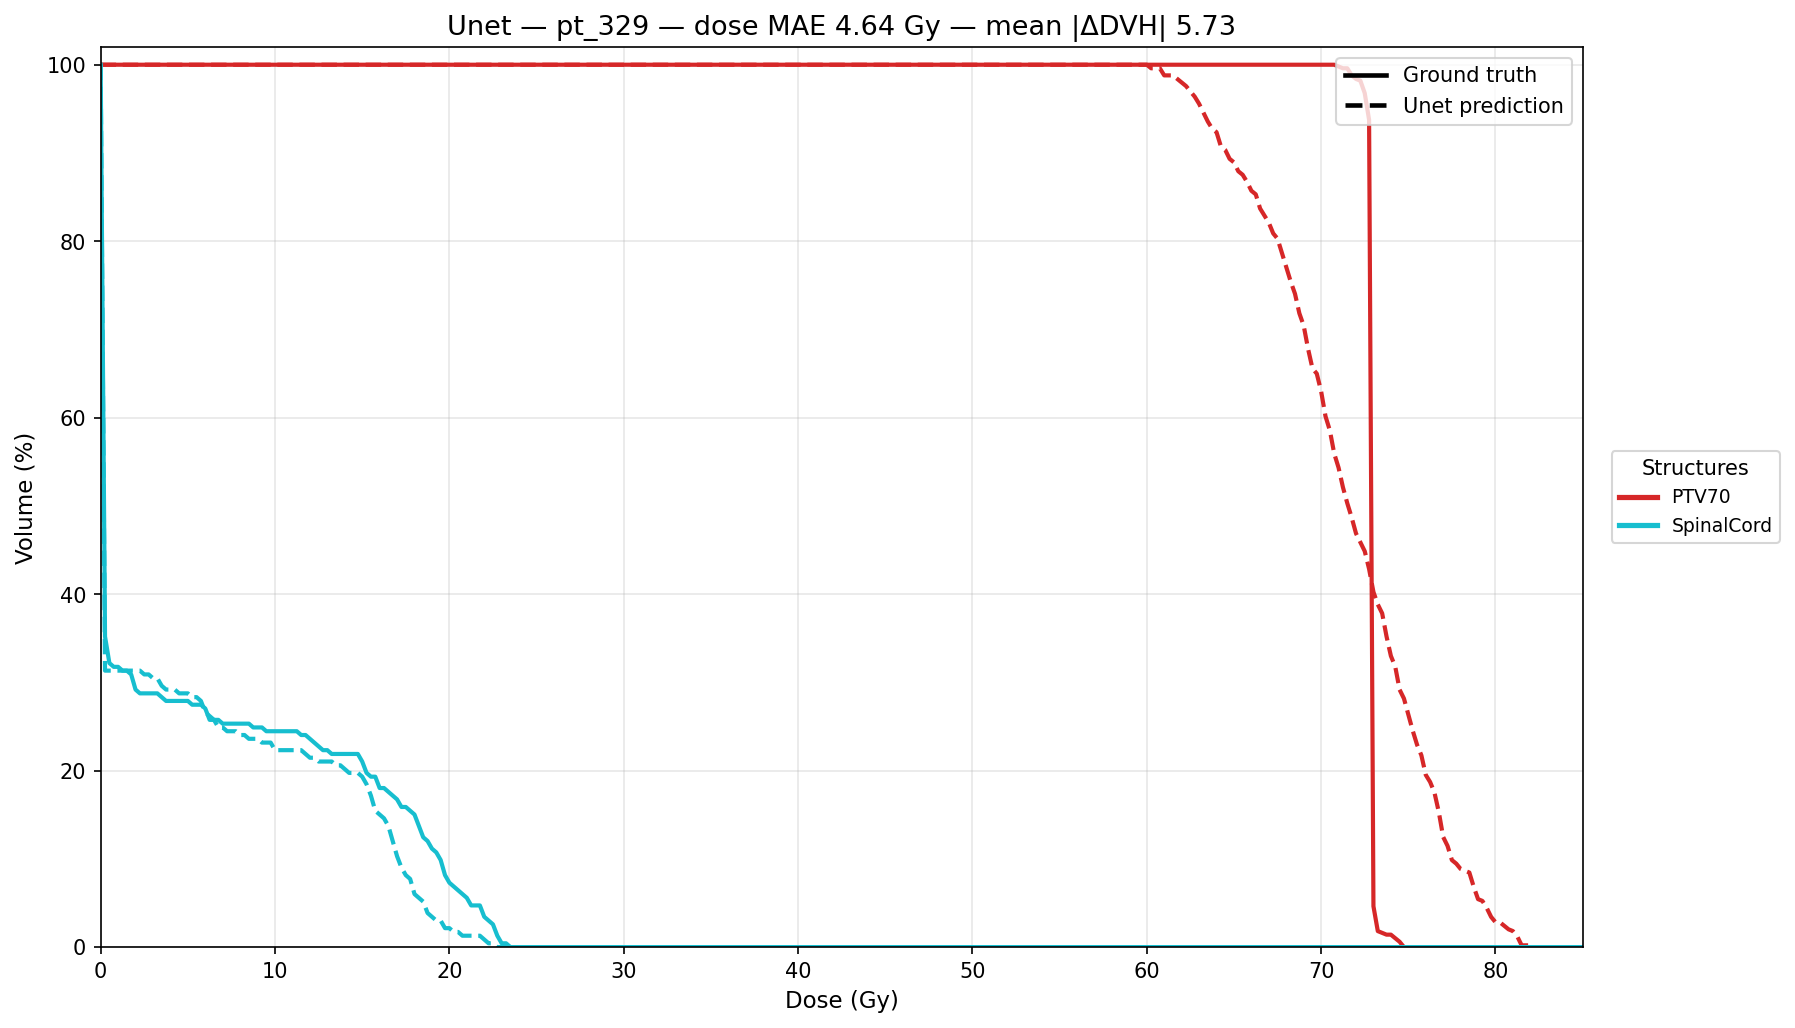
\includegraphics[width=0.493\textwidth]{Figures/pt329-unet.png}\hfill
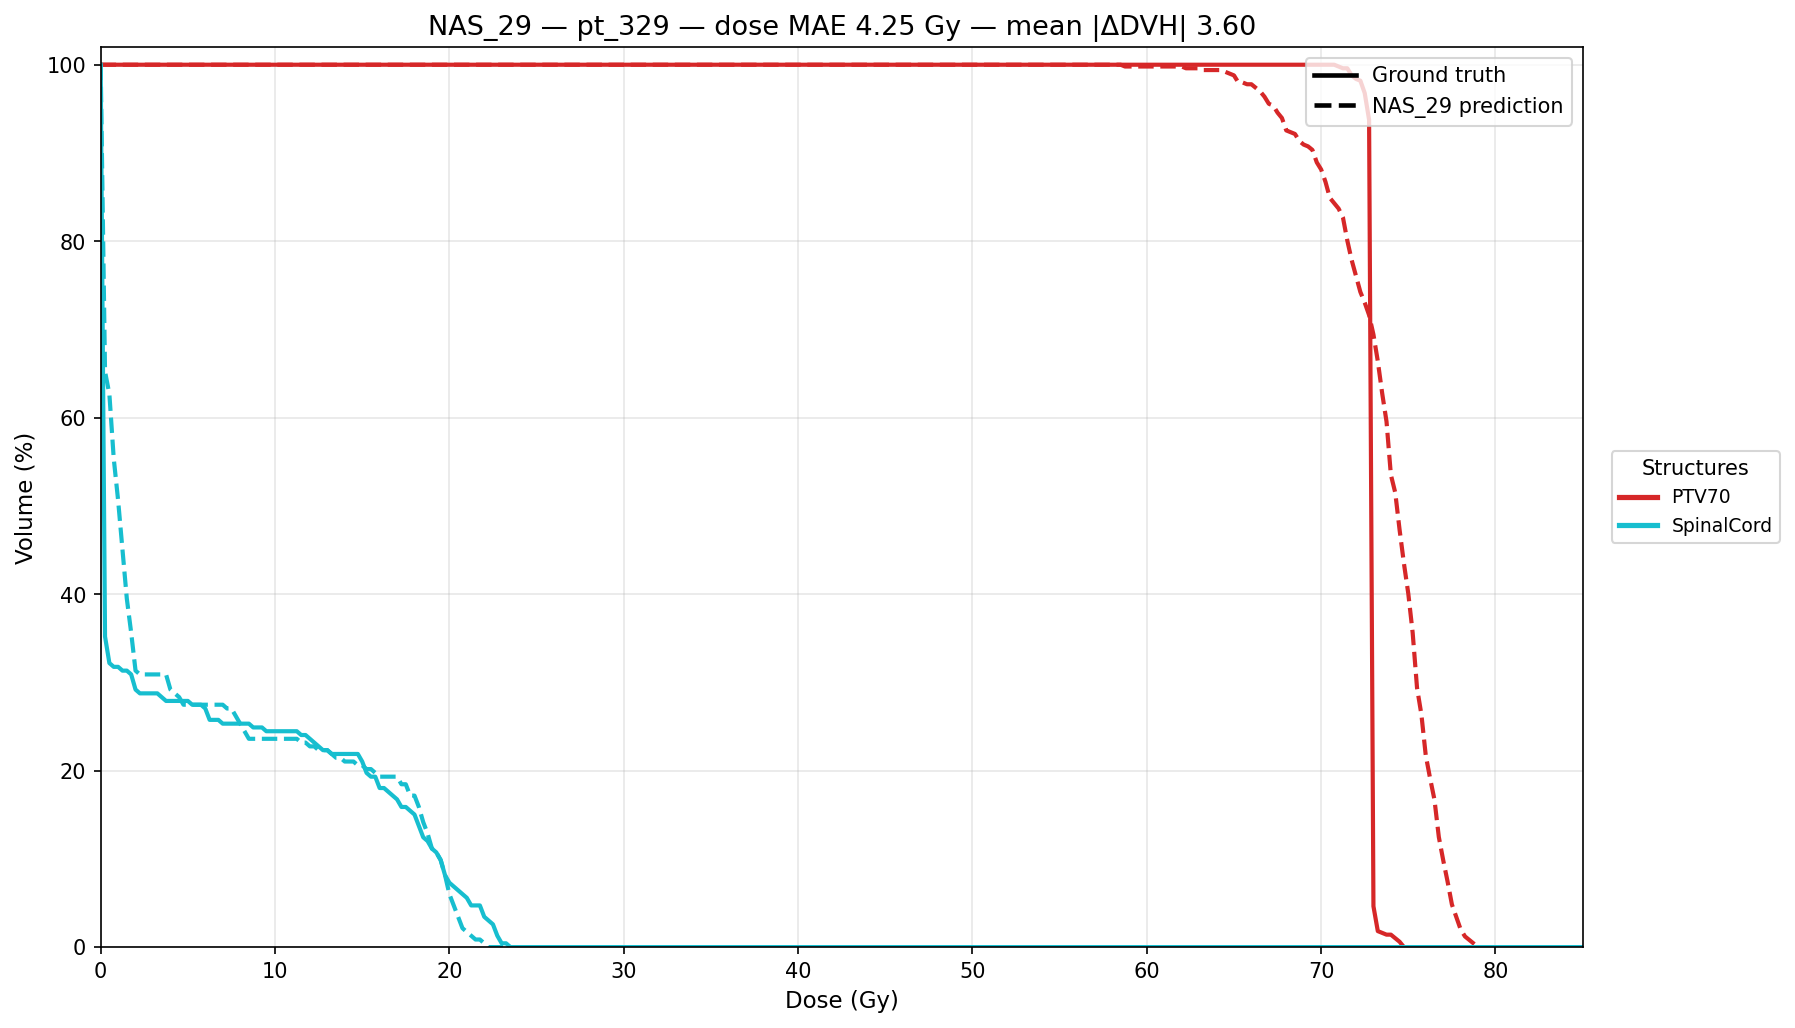
\includegraphics[width=0.493\textwidth]{Figures/pt329-nas29.png}
\caption{患者 329 的累积 DVH，左为 U-Net，右为 NAS-29。每图在同一坐标内叠加 PTV70（红）和脊髓（青）；实线为参考，虚线为预测。横轴为剂量（Gy），纵轴为体积分数（\%）。在 95\% 靶体积处，NAS-29 更接近参考曲线的陡降段。本例因两模型差异较大而回顾性选出。}
\label{fig:dvh}
\end{figure*}

\subsection{评价终点与汇总方式}
剂量分数为各患者 $e_i$ 的算术平均，每名患者等权。对每个已勾画 PTV，比较 $D_1$、$D_{95}$ 和 $D_{99}$，其中 $D_x$ 表示至少 $x$\% 的靶体积接受的剂量。对每个已勾画 OAR，比较平均剂量及最高剂量 0.1 立方厘米组织的近最大剂量，体积换算使用实际体素间距。每项比较产生一个以 Gy 为单位的绝对误差。汇总 DVH 分数对每个有效的患者、结构、终点条目等权，故勾画结构较多的患者权重较高。

我们另计算每名患者的平均 DVH 终点误差，并描述 100 名患者的分布。汇总 DVH 标准差描述 1,783 个指标条目间的变异，患者级标准差则描述个体间变异。下文均采用以 $n$ 为分母的总体标准差，范围为观察到的最小、最大值。计算差值前先按患者、结构和终点匹配两模型的记录。





\subsection{患者级与分结构结果}
与 U-Net 相比，NAS-29 的平均剂量误差降低 0.098 Gy（3.7\%），汇总 DVH 误差降低 0.146 Gy（8.1\%）（表~\ref{tab:results}）。100 名患者中，73 人的剂量误差在 NAS-29 上更低，60 人的患者内平均 DVH 误差在 NAS-29 上更低。为估计患者间的不确定性，我们以固定种子 29 进行 10,000 次配对自助重抽样，每次抽取 100 名患者。重新计算汇总分数时，每名抽中患者贡献其全部可用 DVH 条目。剂量和 DVH 误差降幅的 95\% 百分位区间分别为 0.050--0.146 Gy 和 0.064--0.230 Gy。两个区间均以本次训练所得的两个检查点为条件。

全部 100 名测试患者均有 PTV70 轮廓。在其三个终点中，$D_{95}$ 的平均绝对误差降幅最大，从 1.876 Gy 降至 1.409 Gy（表~\ref{tab:endpoints}）。两侧腮腺平均剂量的预测也有所改善。脊髓近最大剂量则呈现相反趋势：在勾画了脊髓的 88 名患者中，平均绝对误差增加了 0.329 Gy。即使两项汇总分数均有利于同一模型，按终点报告误差与有效病例数仍能揭示这一权衡。

\begin{table}[t]
\centering\small
\begin{tabular}{lrrr}
\toprule
结构与终点 & $n$ & U-Net & NAS-29\\
\midrule
PTV70 $D_1$ & 100 & 1.868 & 1.744\\
PTV70 $D_{95}$ & 100 & 1.876 & 1.409\\
PTV70 $D_{99}$ & 100 & 2.141 & 1.863\\
脑干 $D_{0.1\mathrm{cc}}$ & 89 & 2.712 & 2.418\\
脊髓 $D_{0.1\mathrm{cc}}$ & 88 & 1.887 & 2.216\\
左腮腺平均剂量 & 98 & 1.665 & 1.450\\
右腮腺平均剂量 & 99 & 1.561 & 1.389\\
\bottomrule
\end{tabular}
\caption{部分靶区与危及器官终点的平均绝对误差（Gy）。每行的两模型均使用相同的 $n$ 名患者。}
\label{tab:endpoints}
\end{table}



\subsection{Visualization Analysis}
图~\ref{fig:dvh} 将两种模型预测的累积 DVH 分别与同一组参考曲线比较。在固定体积分数处，预测曲线与参考曲线的水平间距即对应终点的绝对剂量误差。为展示差异，我们在两项分数均有利于 NAS-29 的患者中，选取平均 DVH 误差降幅最大者。患者 329 有两个已勾画结构和五个 DVH 终点。其剂量误差由 4.643 Gy 降至 4.253 Gy，平均 DVH 误差由 5.729 Gy 降至 3.599 Gy。两模型在该患者上的剂量误差均高于各自的队列均值。

两组曲线最明显的差异出现在 PTV70 的陡降段。在靶体积的 95\% 处，参考剂量为 72.71 Gy，U-Net 和 NAS-29 对应的剂量分别为 63.18 Gy 和 67.46 Gy。在 $D_{99}$ 处，绝对误差同样下降，由 10.75 Gy 减至 6.95 Gy。两模型均低估了靶区覆盖剂量。对于脊髓受照剂量最高的 0.1 立方厘米，参考剂量为 22.77 Gy，U-Net 和 NAS-29 分别预测为 21.99 Gy 和 21.42 Gy。因此，本例整体 DVH 误差的降低主要来自靶区预测与参考剂量更为接近。

\section{结果解释与局限}
在相同训练方案下，一种 SearchedNet 配置的两项基准误差均低于固定 U-Net。此次比较评价的是两个完整预测器。二者在参数量和多个算子上均有差异，因而不能将观测到的改善归因于某个特定编码算子或上采样算子。NAS-29 在两次训练之前已被指定。评估智能体的贡献需要另一组对照，使不同选型策略使用相同的架构空间和计算预算。

拟议的训练清单对照也有局限。在优化更新次数固定时，排除部分病例会提高其余患者被抽取的期望次数。表现变化可能同时反映病例曝光次数、标注质量及病例组成的变化，因此应同时报告更新次数和每例曝光次数。复用验证集筛选架构、选择检查点和比较训练清单，也限制了最佳验证分数的解释。由于本次 OpenKBP 比较已影响搜索方案的设计，独立的外部测试尤为重要。

\section{未来工作}
首项实现研究将评估审查者能否根据记录的输入和输出重建每次选型决策。我们拟保存控制器版本、提示词及解码设置、工具版本、硬件测量、种子、清单、实际优化器参数组和被淘汰的试验。审查者将把一项声称的改善追溯至匹配对照，并识别因多个算子同时改变而仍未得到验证的解释。在 Bridge 工作环节中，我们计划以事件模式和患者 329 的 DVH 为例，了解医学物理师和人工智能研究者在质疑一次模型选择时需要哪些记录。

我们将比较完整智能体、固定 U-Net、固定 NAS-29，以及在相同预算和搜索空间内不使用队列测量的采样搜索。消融实验将分别检验数据筛选、证据引导的提案和调参的作用；通过多个训练种子评估选型稳定性、计算成本，以及排除病例的提案获得匹配对照支持的频率。除 U-Net 和 SearchedNet 外，我们还将用相同的数据划分和评价终点，比较可配置的 nnDoseNet 框架与利用距离信息的扩散模型 DoseDiff\citep{nndose,dosediff}。若其中的框架在相近计算资源下能更准确地预测靶区或器官剂量，我们将进一步检验：允许智能体跨框架选型，能否提高整体预测精度。

外部评价将纳入来自其他机构和解剖部位的独立队列，包括前列腺放疗。迁移前将统一处方定义、轮廓定义和采集几何，并在选型前锁定各外部测试集。对体积较小或勾画较少的结构，我们将分别报告误差和覆盖情况，并请临床评审者检查体素剂量分数与 DVH 分数结论不一致的病例。这样既能检验模型能否推广至新患者，也能检验某个终点恶化时，能否追溯选型所依据的证据。

\paragraph{人工智能辅助说明} OpenAI Codex（GPT-6）协助论文起草、文献检索、已有实验结果制表和 LaTeX 排版。文中剂量预测由两个已训练的神经网络生成，所设计的语言模型控制器尚未在这些实验中运行。

\bibliography{references}
\end{document}
